% Author:: Sebastien Badia (<seb@sebian.fr>)
% Date:: 2014-04-02 01:36:20 +0200
% vi: set ft=tex :

\section{Cloud computing}
\begin{frame}{Outline}
    \tableofcontents[currentsection,hideallsubsections]
\end{frame}
\subsection{Definition}

\begin{frame}{Cloud computing}
\begin{block}{Definition}
Cloud computing is a model for enabling convenient, on-demand network access to a shared pool of configurable computing resources.
\end{block}
\begin{itemize}
  \item \textbf{On Demand}: Resources are dynamically created.
  \item \textbf{Multi-tenant}: Resources are shared between users.
  \item \textbf{Broad network access}: Network, standard mechanisms
  \item \textbf{Elasticity}: Infrastructure is flexible (grow/reduce).
  \item \textbf{Measured service}: Users pay what they use.
\end{itemize}
\end{frame}

\subsection{Cloud layers}
\begin{frame}{Cloud computing}
  \begin{textblock}{}(11,2)
      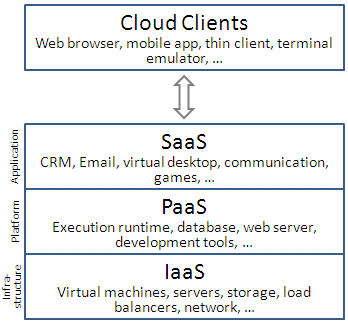
\includegraphics[width=8em]{img/Cloud_computing_layers}
  \end{textblock}
  \begin{itemize}
    \item Service models by the NIST\footnote{National Institute of Standards and Technology} (24 July 2011)
      \begin{itemize}
        \item Infrastructure as a service (IaaS)
        \medskip
        \item Platform as a service (PaaS)
        \medskip
        \item Software as a service (SaaS)
        \medskip
      \end{itemize}
    \item XaaS, a comprehensive taxonomy model
      \begin{itemize}
        \item Database as a service (DaaS)
        \medskip
        \item Network as a service (NaaS)
        \medskip
        \item …
      \end{itemize}
  \end{itemize}
\end{frame}
